%%%%%%%%%%%%%%%%%%%%%%%%%%%%%%%%%%%%%%%%%%%%%%%%%%%%%%%%
% Este é um documento que servirá de modelo para
% os relatórios feitos na disciplina Laboratório de Circuitos Lógicos
% 2020-2
%%%%%%%%%%%%%%%%%%%%%%%%%%%%%%%%%%%%%%%%%%%%%%%%%%%%%%%%%

%%%%%%%%%%%%%%%%%%%%%%%%%%%%%%%%%%%%%%%%%%%%%%%%%%%%%%%%%
% Use os diferentes diretórios para colocar os relatórios de cada experimento, deste modo vc consegue manter um histórico e todo material organizado em apenas um local.
% Lembre-se de mudar o Main Document no Menu!!!

\documentclass[12pt]{article}

\usepackage{sbc-template}
\usepackage[brazil,american]{babel}
\usepackage[utf8]{inputenc}

\usepackage{graphicx}
\usepackage{url}
\usepackage{float}
\usepackage{listings}
\usepackage{color}
\usepackage{todonotes}
\usepackage{algorithmic}
\usepackage{algorithm}
\usepackage{hyperref}
\usepackage{amsmath}
\usepackage{graphicx}
\usepackage{array}
\usepackage{mwe}
\usepackage[shortlabels]{enumitem}

\usepackage{xcolor}
\usepackage{listings}
\definecolor{vgreen}{RGB}{104,180,104}
\definecolor{vblue}{RGB}{49,49,255}
\definecolor{vorange}{RGB}{255,143,102}

\lstdefinestyle{verilog-style}
{
    language=Verilog,
    basicstyle=\small\ttfamily,
    keywordstyle=\color{vblue},
    identifierstyle=\color{black},
    commentstyle=\color{vgreen},
    numbers=left,
    numberstyle=\tiny\color{black},
    numbersep=10pt,
    tabsize=8,
    moredelim=*[s][\colorIndex]{[}{]},
    literate=*{:}{:}1
}

\makeatletter
\newcommand*\@lbracket{[}
\newcommand*\@rbracket{]}
\newcommand*\@colon{:}
\newcommand*\colorIndex{%
    \edef\@temp{\the\lst@token}%
    \ifx\@temp\@lbracket \color{black}%
    \else\ifx\@temp\@rbracket \color{black}%
    \else\ifx\@temp\@colon \color{black}%
    \else \color{vorange}%
    \fi\fi\fi
}
\makeatother

\usepackage{trace}

\sloppy


\title{Experimento 6\\
Implementação de Circuitos Combinacionais com Multiplexadores}

\author{Matheus Cardoso de Souza, 202033507\\
        Ualiton Ventura da Silva, 202033580\\
        Grupo G42
}

%%%% LEMBRE-SE DE MUDAR O GRUPO NA LINHA ABAIXO!!!!! %%%%%%
\address{Dep. Ciência da Computação -- Universidade de Brasília (UnB)\\
  CIC0231 - Laboratório de Circuitos Lógicos
  \email{matheus-cardoso.mc@aluno.unb.br, 202033580@aluno.unb.br}
}

\begin{document}
\maketitle

\selectlanguage{american}
 \begin{abstract}
   The current report aims to show the elaboration, implementation and analysis
   of logic circuits using multiplexers and decoders as main the main logic
   components. Furthermore, it was explored the use of more advanced tools to
   describe the hardware, using the \emph{SystemVerilog} language for more
   assertive, pratical and scalable representation of complex systems.
 \end{abstract}

\selectlanguage{brazil}
 \begin{resumo}
   O presente relatório tem como objetivo a elaboração, implementação e análise
   de circuitos lógicos utilizando-se multiplexadores e decodificadores como os
   principais componentes lógicos. Além disso, foi explorado o uso de
   ferramentas mais avançadas para a descrição de hardware, valendo-se da
   linguagem \emph{SystemVerilog} para uma representação assertiva, prática e
   escalável de sistemas complexos.
 \end{resumo}


\section{Introdução}\label{sec:Introducao}

Como nesse relatório faremos uso de forma extensa de multiplexadores e
decodificadores, cabe inicialmente uma explanação breve sobre esses circuitos
lógicos, bem como suas propriedades e aplicações.


Multiplexadores (ou \emph{mux}) são circuitos combinacionais capazes de mapear
$2^{N}$ entradas para apenas $1$ saída, sendo, portanto, conhecidos também como
\emph{seletores de dados}. No caso, quando existem $2^{N}$ dados de entrada, é
requerido um total de $N$ seletores para satisfatoriamente cumprir o mapeamento
$2^{N} \rightarrow 1$.

Na figura~\ref{fig:mux.png} (fonte:~\cite{isc_mod3}) é possível
entender conceitualmente o funcionamento de um multiplexador, e, na
figura~\ref{fig:mux_wiki.png} (fonte:~\cite{wiki_mux}) é possível visualizar com
maiores detalhes a implementação por circuitos lógicos de um multiplexador.

\begin{figure}[H]
    \centering
    \begin{minipage}{0.45\textwidth}
      \centering
      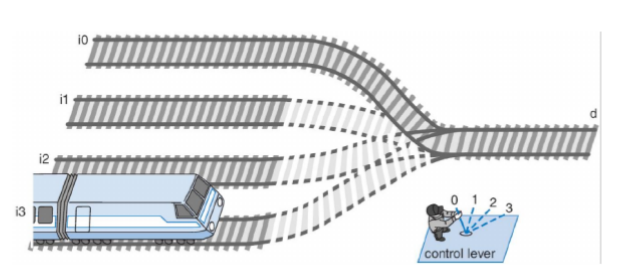
\includegraphics[width=0.9\textwidth]{Exp06/Images/mux.png}
      \caption{Como um multiplexador funciona}\label{fig:mux.png}
    \end{minipage}\hfill
    \begin{minipage}{0.45\textwidth}
      \centering
      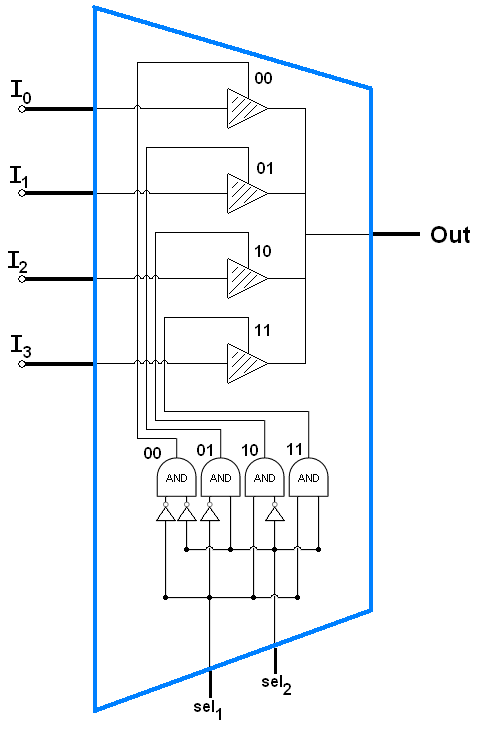
\includegraphics[width=0.5\textwidth]{Exp06/Images/mux_wiki.png}
      \caption{Implementação de um multiplexador}\label{fig:mux_wiki.png}
    \end{minipage}\hfill
\end{figure}

Um dos usos de multiplexadores é na economia de conexões ao longo de um único
canal, conectando o único output do multiplexador com o único input do
demultiplexador. Dessa forma, o benefício é que seria possível reduzir o custo
de implementação física de múltiplos canais para cada uma das fontes de dados no
circuito. Pode-se observar como funcionaria um circuito desse na
figura~\ref{fig:mux_demux.png}

\begin{figure}[H]
  \centering
  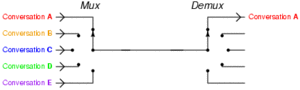
\includegraphics[width=0.5\textwidth]{Exp06/Images/mux_demux.png}
  \caption{Uma das aplicações de um Multiplexador}\label{fig:mux_demux.png}
\end{figure}

Considerando agora os demultiplexadores, podemos afirmar que eles são
basicamente a ``\emph{função inversa}'' dos multiplexadores, convertendo $1$
input em $2^{N}$ outputs, e possuindo $N$ seletores. O diagrama básico de um
demultiplexador pode ser visto na figura~\ref{fig:demux.png}
(fonte:~\cite{web_demux}).

\begin{figure}[H]
  \centering
  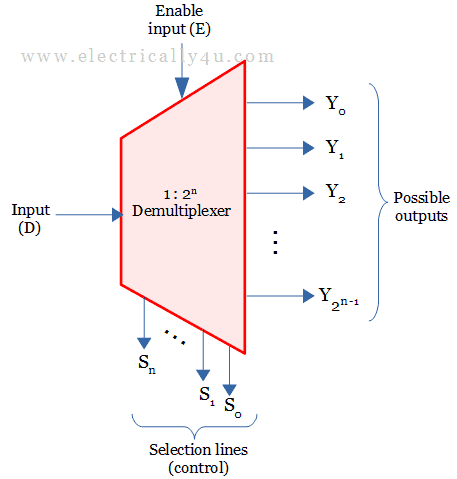
\includegraphics[width=0.4\textwidth]{Exp06/Images/demux.png}
  \caption{Diagrama de um demultiplexador}\label{fig:demux.png}
\end{figure}

Por fim, os decodificadores. Podemos dizer que são muito semelhantes aos
demultiplexadores, cabendo a ressalva de que uma diferença significativa entre
os dois é que decodificadores não possuem o seletor entre ativo e inativo, já os
demultiplexadores podem estar no estado ativo ou inativo. Um diagrama de um
codificador pode ser visto na figura~\ref{fig:decoder.png}
(fonte:~\cite{web_decoder}).

\begin{figure}[H]
  \centering
  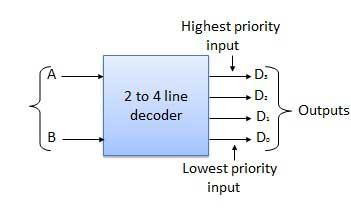
\includegraphics[width=0.5\textwidth]{Exp06/Images/decoder.png}
  \caption{Diagrama de um decodificador}\label{fig:decoder.png}
\end{figure}


Agora, após uma breve explicação das propriedades de multiplexadores,
demultiplexadores e decodificadores, podemos considerar o uso deles para a
implementação de circuitos lógicos mais complexos, e bem importantes no dia a
dia. Um exemplo de circuito lógico muito importante, e de presença praticamente
ubíqua nos circuitos computacionais atuais são os circuitos somadores,
responsáveis por operações simples mas básicas e necessárias a toda computação
de números. Tais circuitos são responsáveis por somar dois bits \textbf{A} e
\textbf{B}, (possivelmente considerando um carry-in ``\textbf{Cin}''), e
resultando na soma \textbf{S} e, possivelmente, no carry-out ``\textbf{Cout}''.
Esse circuito simples é a base para muitos cálculos algébricos realizados em
praticamente todo ciclo de clock de um computador moderno. Outra aplicação
importante que multiplexadores, demultiplexadores e decodificadores permitem é a
implementação de funções genéricas complexas de forma relativamente simples.
Essas duas aplicações serão abordadas de forma mais técnica e profunda nos
tópicos seguintes.


\subsection{Objetivos}\label{sec:Objetivos}

Os textos subsequentes deste presente relatório tem por finalidade a elaboração
de circuitos lógicos para implementação de somadores e funções lógicas
arbitráriass valendo-se de circuitos combinacionais como multiplexadores e
decodificadores. A montagem desses circuitos se dará tanto no nível de
implementação manual dos circuitos e portas lógicas, bem como o uso da linguagem
\emph{SystemVerilog}.


\subsection{Materiais}
\label{sec:Materiais}
Em função da natureza do ensino a distância, os presentes experimentos não foram
realizados usando-se materiais e equipamentos físicos, mas sim emulados por meio
do
\href{https://www.intel.com/content/www/us/en/software/programmable/quartus-prime/download.html}{Quartus-II}.

A seguir estão enumerados os materiais utilizados:
\begin{itemize}
    \item Software Quartus-II versão 13.0 SP1
    \item Multiplexadores
    \item Decodificadores
    \item Portas Lógicas \textbf{NOT}, \textbf{Buffer}
\end{itemize}

\section{Procedimentos}
\label{sec:Procedimentos}
% \setcounter{subsection}{-1}

Passaremos a apresentar os experimentos requeridos.

% 2.1
\subsection{Elaboração de Somador Completo desenhando o circuito}\label{sec:2.1}

Para a elaboração do somador requerido no enunciado, precisamos inicialmente
criar o circuito de um multiplexador. Como requisitado, implementaremos um
multiplexador 8x1 usando \emph{SystemVerilog}. O código necessário para criar
tal multiplexador é representado em~\ref{code:mux8}.

\begin{center}
    \begin{lstlisting}[style={verilog-style}]
    module mux8(
        input [7:0] dado,
        input [2:0] escolha,
        output saida
        );

        assign saida = dado[escolha];
    endmodule
    \end{lstlisting}
    \label{code:mux8}
\end{center}

Agora que dispomos do multiplexador necessário para a construção de um somador,
precisamos analisar a tabela verdade da função desejada para construirmos um
circuito adequado.

A tabela verdade desejada do somador está representada
em~\ref{tab:truth_table_full_adder}:

\begin{table}[H]
    \centering
    \caption{Tabela Verdade para o Somador}
    \begin{tabular}{|c|c|c||c|c|}\hline
    \multicolumn{3}{|c||}{Entradas} & \multicolumn{2}{|c|}{Saídas} \\\hline
    \textbf{A} & \textbf{B} & \textbf{Cin} & \textbf{Cout} & \textbf{S} \\\hline
    0 & 0 & 0 & 0 & 0 \\\hline
    0 & 0 & 1 & 0 & 1 \\\hline
    0 & 1 & 0 & 0 & 1 \\\hline
    0 & 1 & 1 & 1 & 0 \\\hline
    1 & 0 & 0 & 0 & 1 \\\hline
    1 & 0 & 1 & 1 & 0 \\\hline
    1 & 1 & 0 & 1 & 0 \\\hline
    1 & 1 & 1 & 1 & 1 \\\hline
    \end{tabular}\label{tab:truth_table_full_adder}
\end{table}

E, de posse da tabela verdade final, podemos agora criar dois circuitos, um para
a função que originará o output de \textbf{Cout} e outra função para o output de
\textbf{S}.

Para o output de \textbf{Cout}, basta implementarmos a seguinte função:

\begin{equation}
f(A,B,Cin) = \overline{A} \cdot B \cdot Cin + A \cdot \overline{B} \cdot Cin + A \cdot B \cdot \overline{Cin} + A \cdot B \cdot Cin
\end{equation}

E, para o output de \textbf{S}, implementaremos a função:

\begin{equation}
g(A,B,Cin) = \overline{A} \cdot \overline{B} \cdot Cin + \overline{A} \cdot B \cdot \overline{Cin} + A \cdot \overline{B} \cdot \overline{Cin} + A \cdot B \cdot Cin
\end{equation}

Seria possível tentarmos minimizar as funções acima, mas, visto que utilizaremos
um multiplexador para a construção do circuito, tal otimização torna-se
desnecessária.

Agora que dispomos de todas as informações necessárias para a construção do
circuito lógico, resta-nos apenas montar o circuito com as portas lógicas, fios
e multiplexadores necessários.

A implementação do circuito requisitado no enunciado pode ser visualizada na
figura~\ref{fig:2_1_Circuit.png}.

\begin{figure}[H]
  \centering
  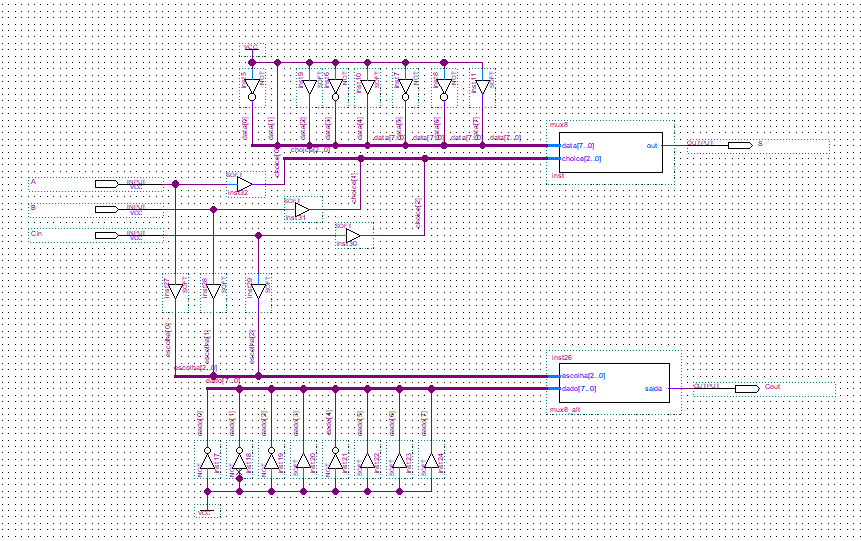
\includegraphics[width=0.9\textwidth]{Exp06/Images/2_1_Circuit.png}
  \caption{Circuito final do somador montado a partir de mapeamento de portas
    lógicas}\label{fig:2_1_Circuit.png}
\end{figure}

Por fim, com o circuito implementado e devidamente demonstrado, passaremos a
apresentar o comportamento efetivo do circuito para todos os possíveis valores
de input de \textbf{A}, \textbf{B} e \textbf{Cin}. O diagrama da simulação
funcional do circuito acima pode ser visto na
figura~\ref{fig:2_1_Functional_Foto.jpg}, e o diagrama da simulação de tempo do
circuito, na figura~\ref{fig:2_1_Timing_Foto.jpg}.

\begin{figure}[H]
  \centering
  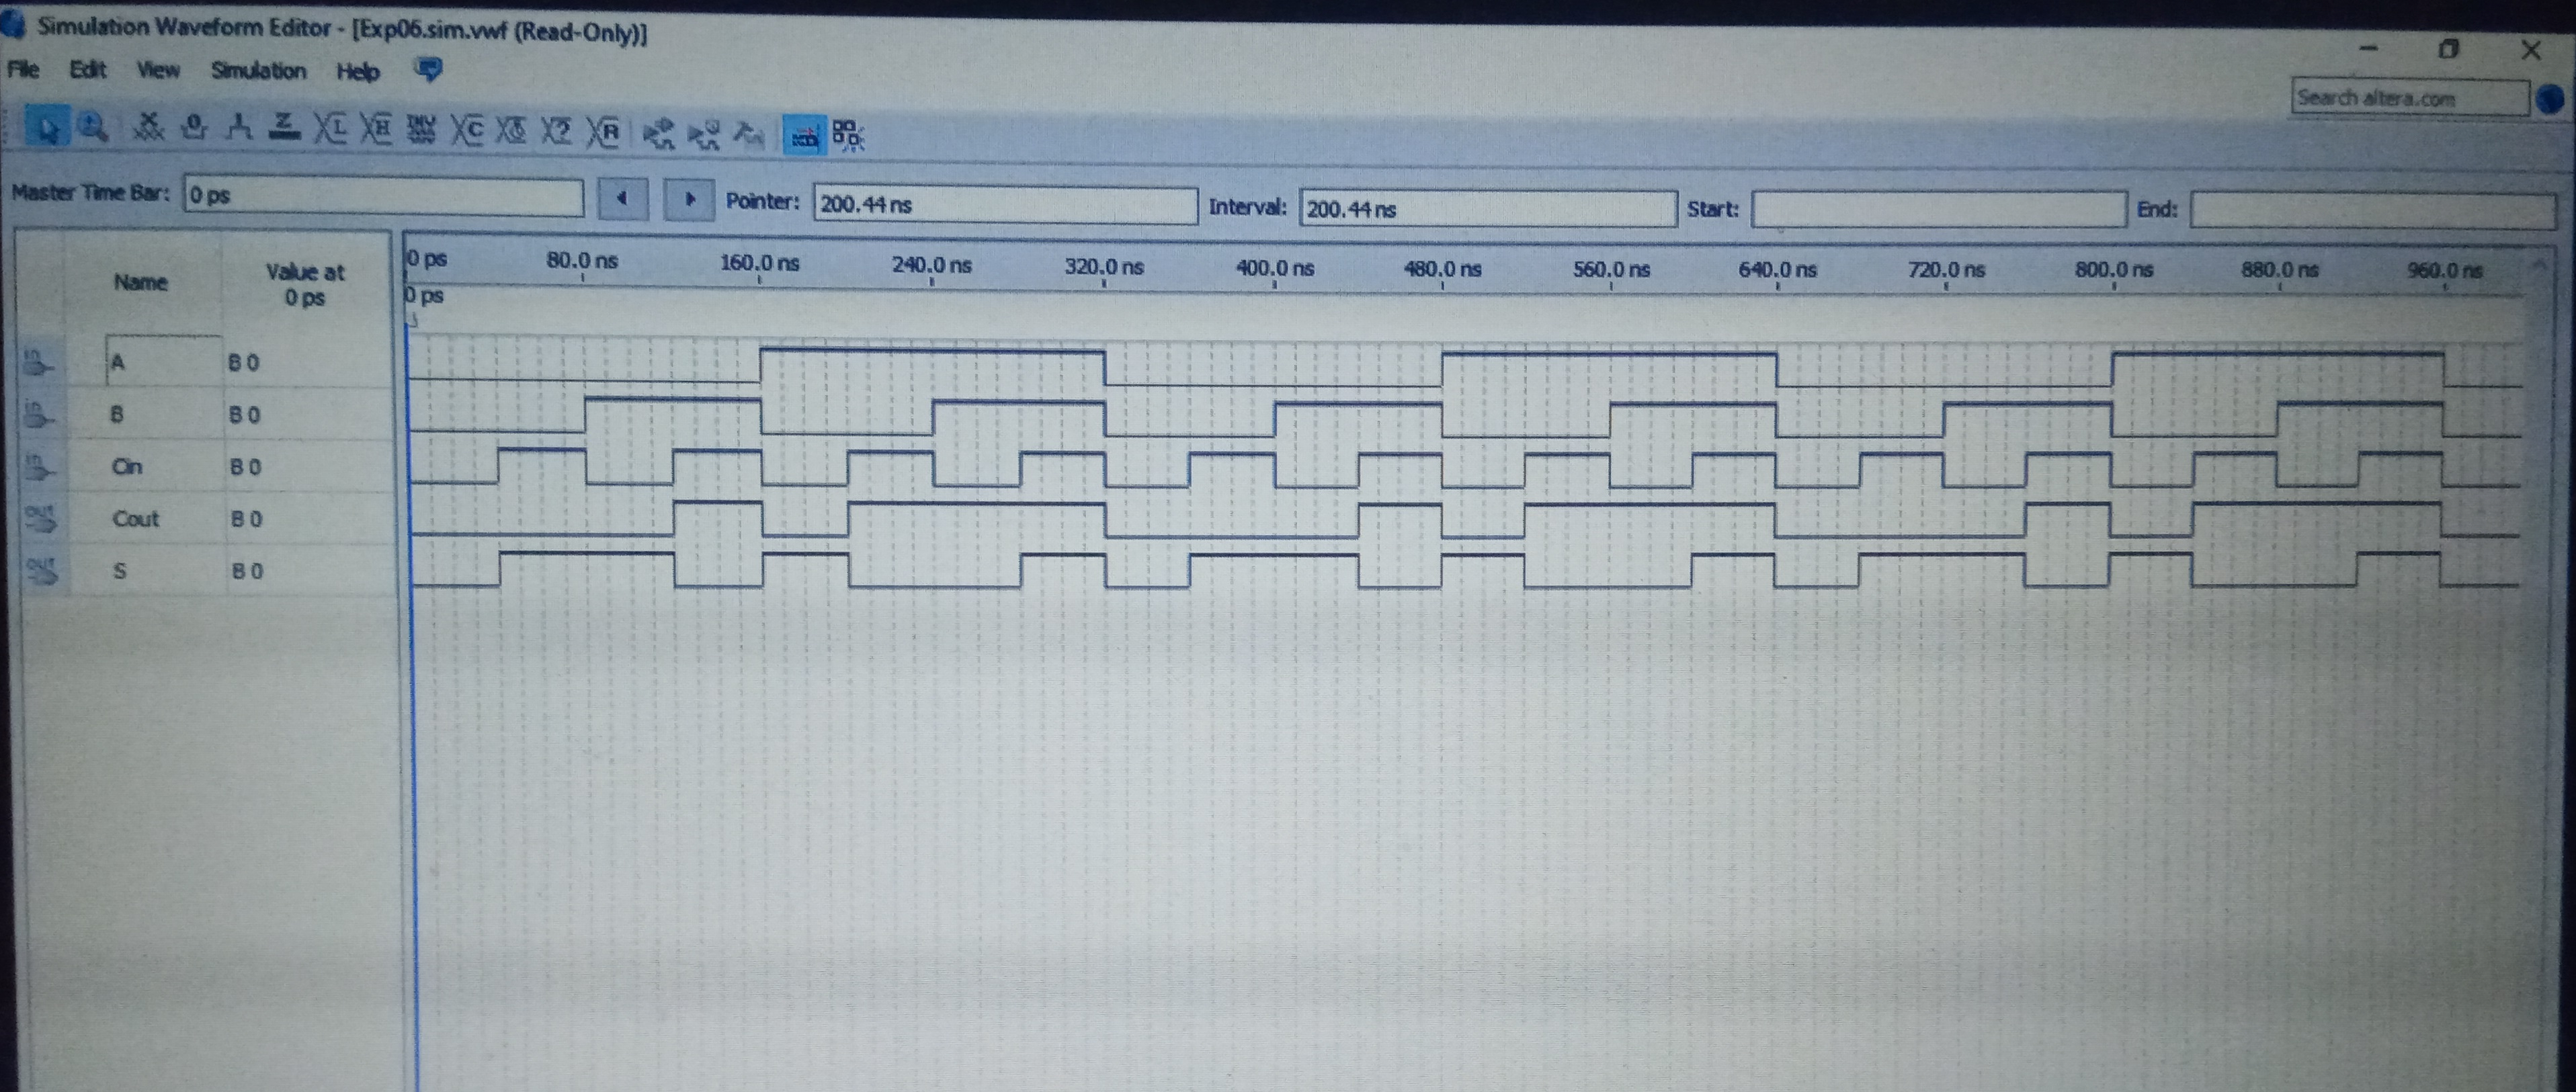
\includegraphics[width=0.9\textwidth]{Exp06/Images/2_1_Functional_Foto.jpg}
  \caption{Diagrama Funcional do Somador}\label{fig:2_1_Functional_Foto.jpg}
\end{figure}

\begin{figure}[H]
  \centering
  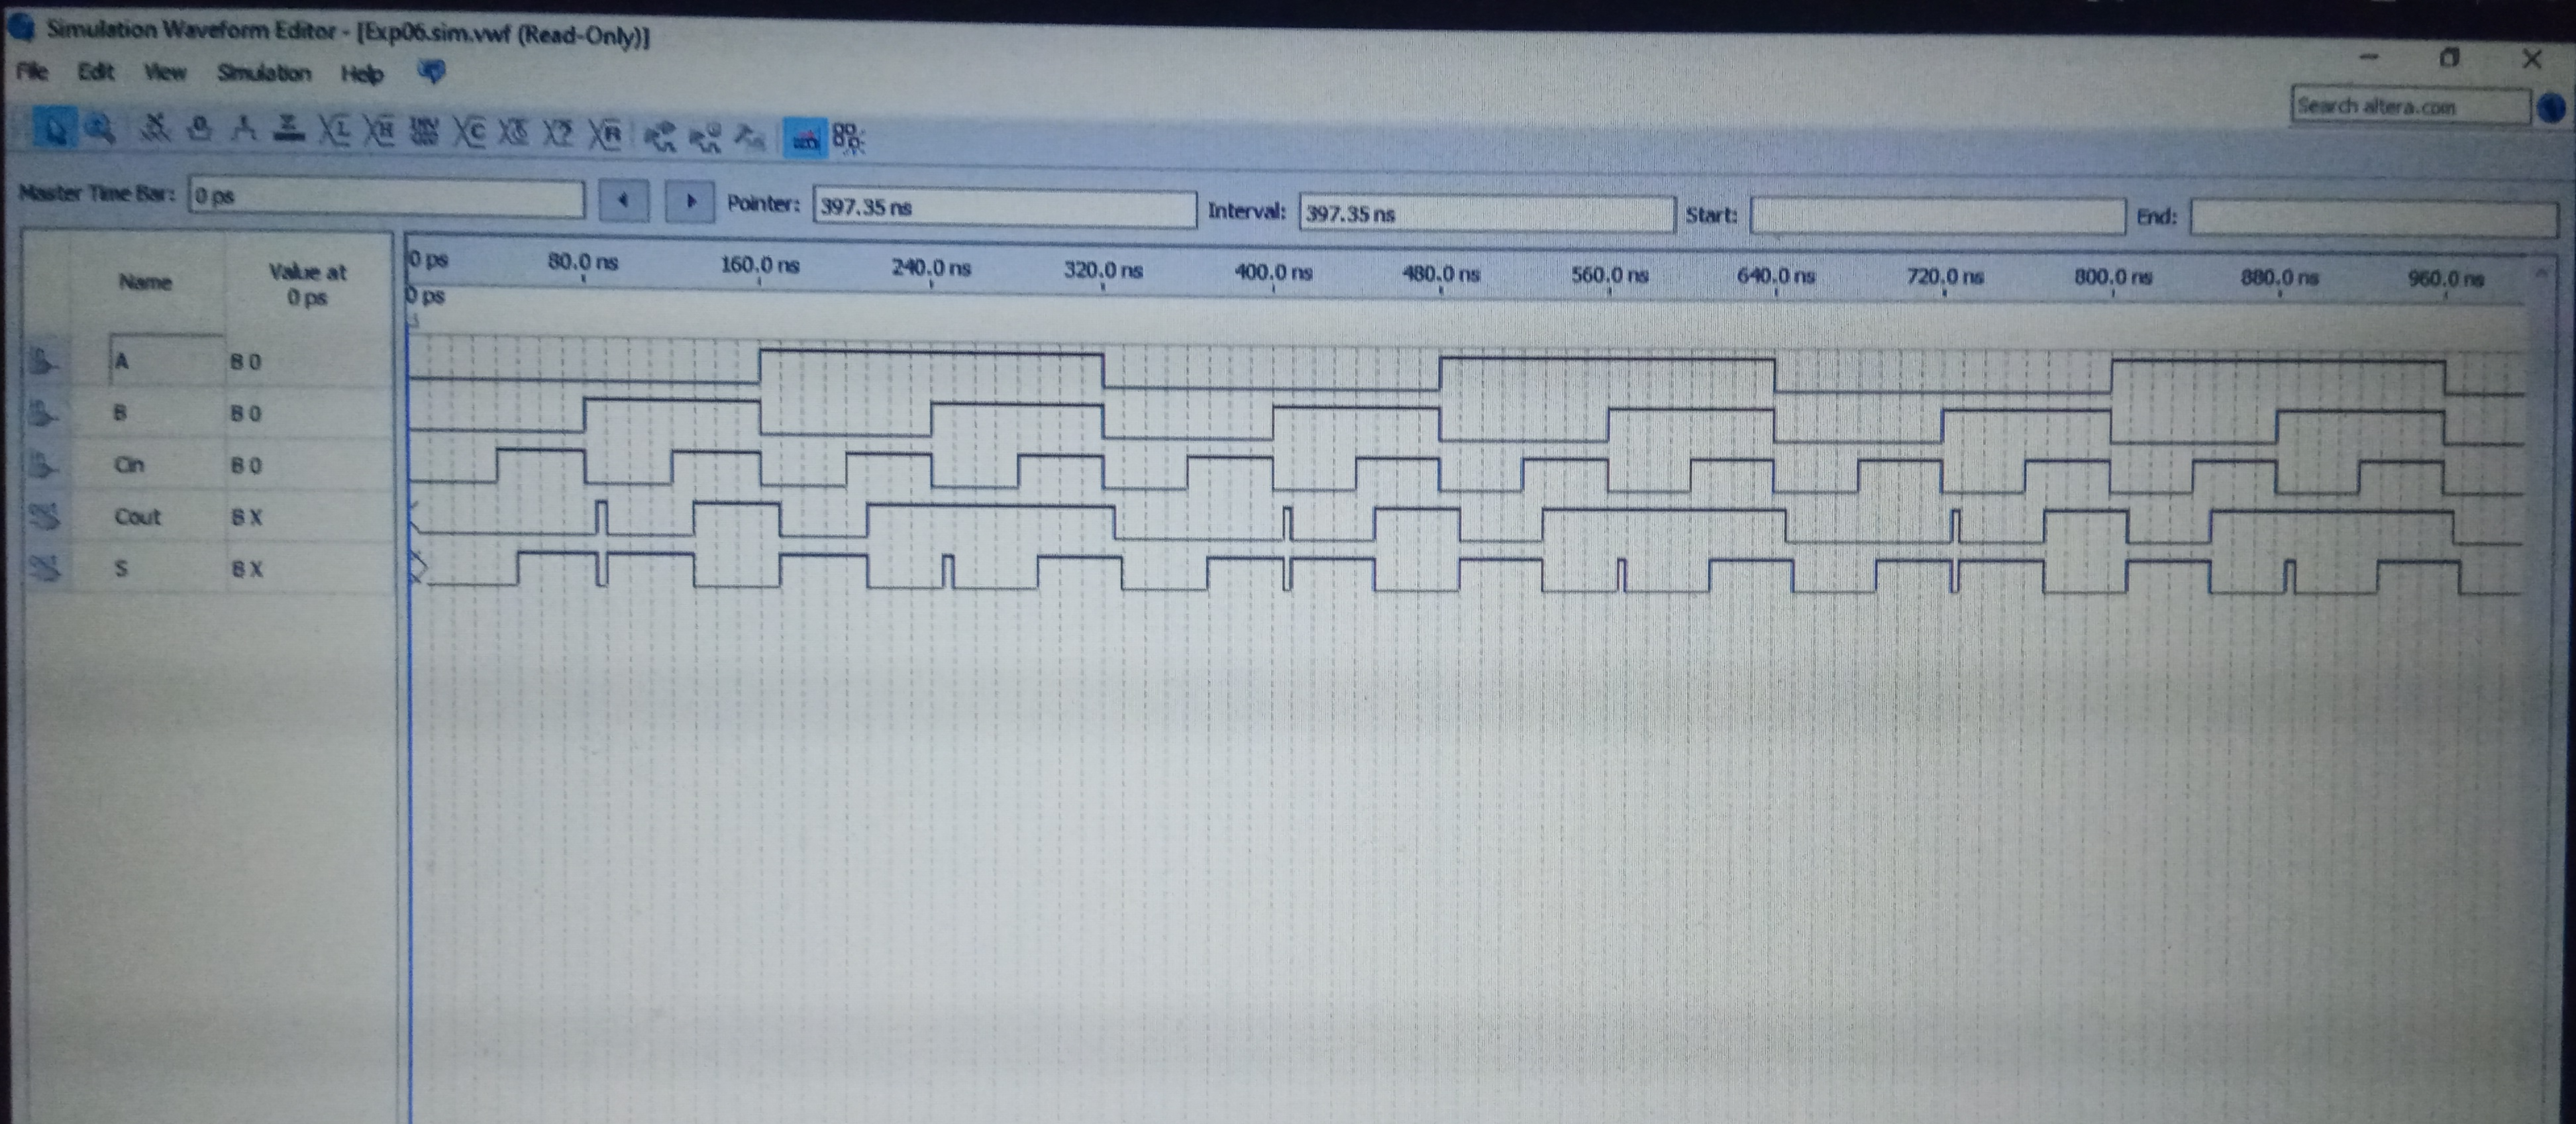
\includegraphics[width=0.9\textwidth]{Exp06/Images/2_1_Timing_Foto.jpg}
  \caption{Diagrama de Tempo do Somador}\label{fig:2_1_Timing_Foto.jpg}
\end{figure}

% 2.2
\subsection{Elaboração de Somador Completo apenas com Verilog}\label{sec:2.2}

Para este tópico, que devemos elaborar um somador usando apenas a descrição em
verilog, vemos quão mais fácil é o desenvolvimento de circuitos lógicos mais
complexos valendo-se de uma linguagem de descrição de hardware adequada.

Para conseguirmos elaborar o somador, basta escrevermos a descrição de um módulo
com o seguinte código:

\begin{center}
    \begin{lstlisting}[style={verilog-style}]
    module full_adder(
        input A,
        input B,
        input Cin,
        output Cout,
        output S
        );

        assign {Cout,S} = A + B + Cin;
    endmodule
    \end{lstlisting}
    \label{code:full_adder}
\end{center}

Com esse código, temos a certeza que a implementação final será a de um somador
totalmente funcional, pois isso é garantido pela linguagem de descrição de
hardware \emph{SystemVerilog}.

Para avaliarmos os diagramas funcional e de tempo do circuito descrito acima,
podemos analizar respectivamente as figuras~\ref{fig:2_2_Functional_Foto.jpg}
e~\ref{fig:2_2_Timing_Foto.jpg}.

\begin{figure}[H]
  \centering
  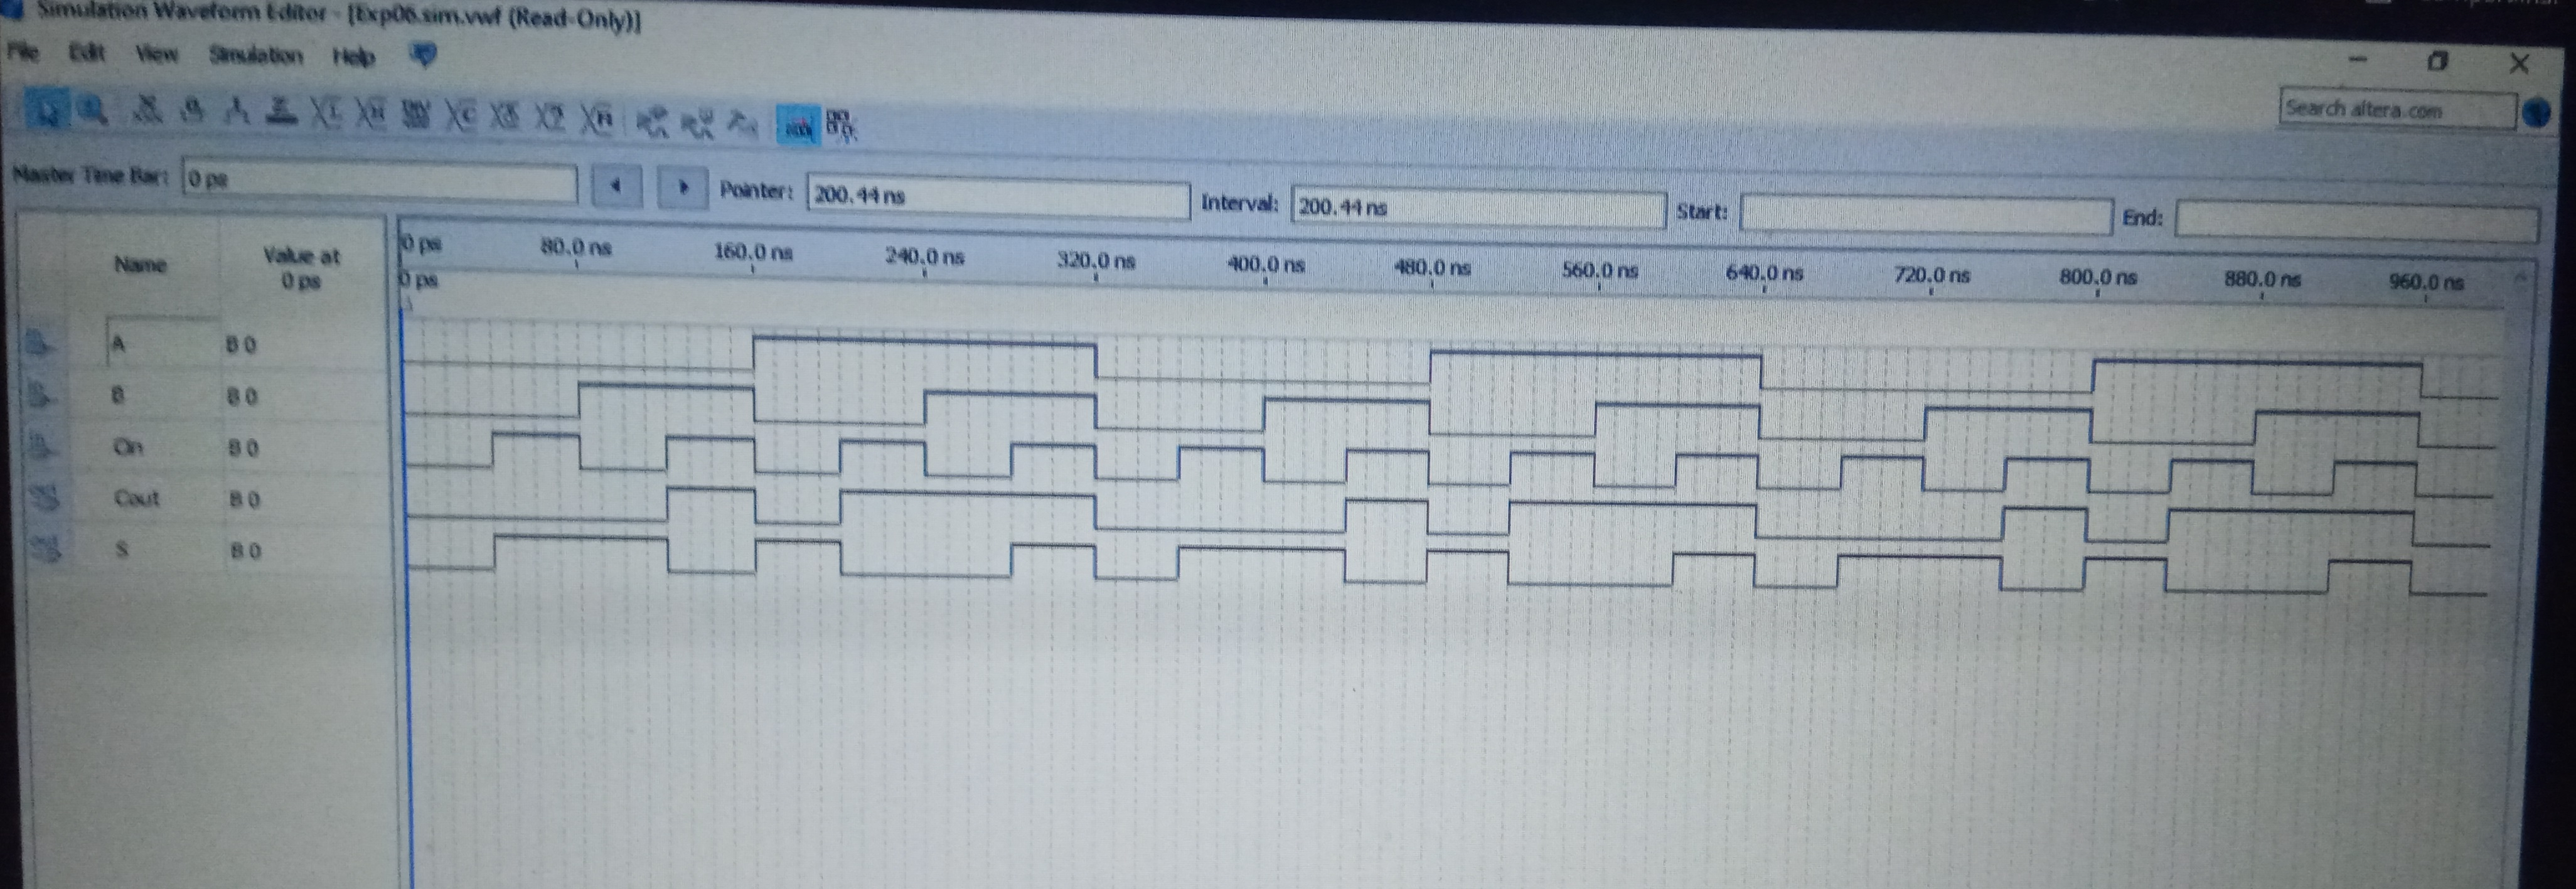
\includegraphics[width=0.9\textwidth]{Exp06/Images/2_2_Functional_Foto.jpg}
  \caption{Diagrama Funcional do Somador implementado com \emph{SystemVerilog}}\label{fig:2_2_Functional_Foto.jpg}
\end{figure}

\begin{figure}[H]
  \centering
  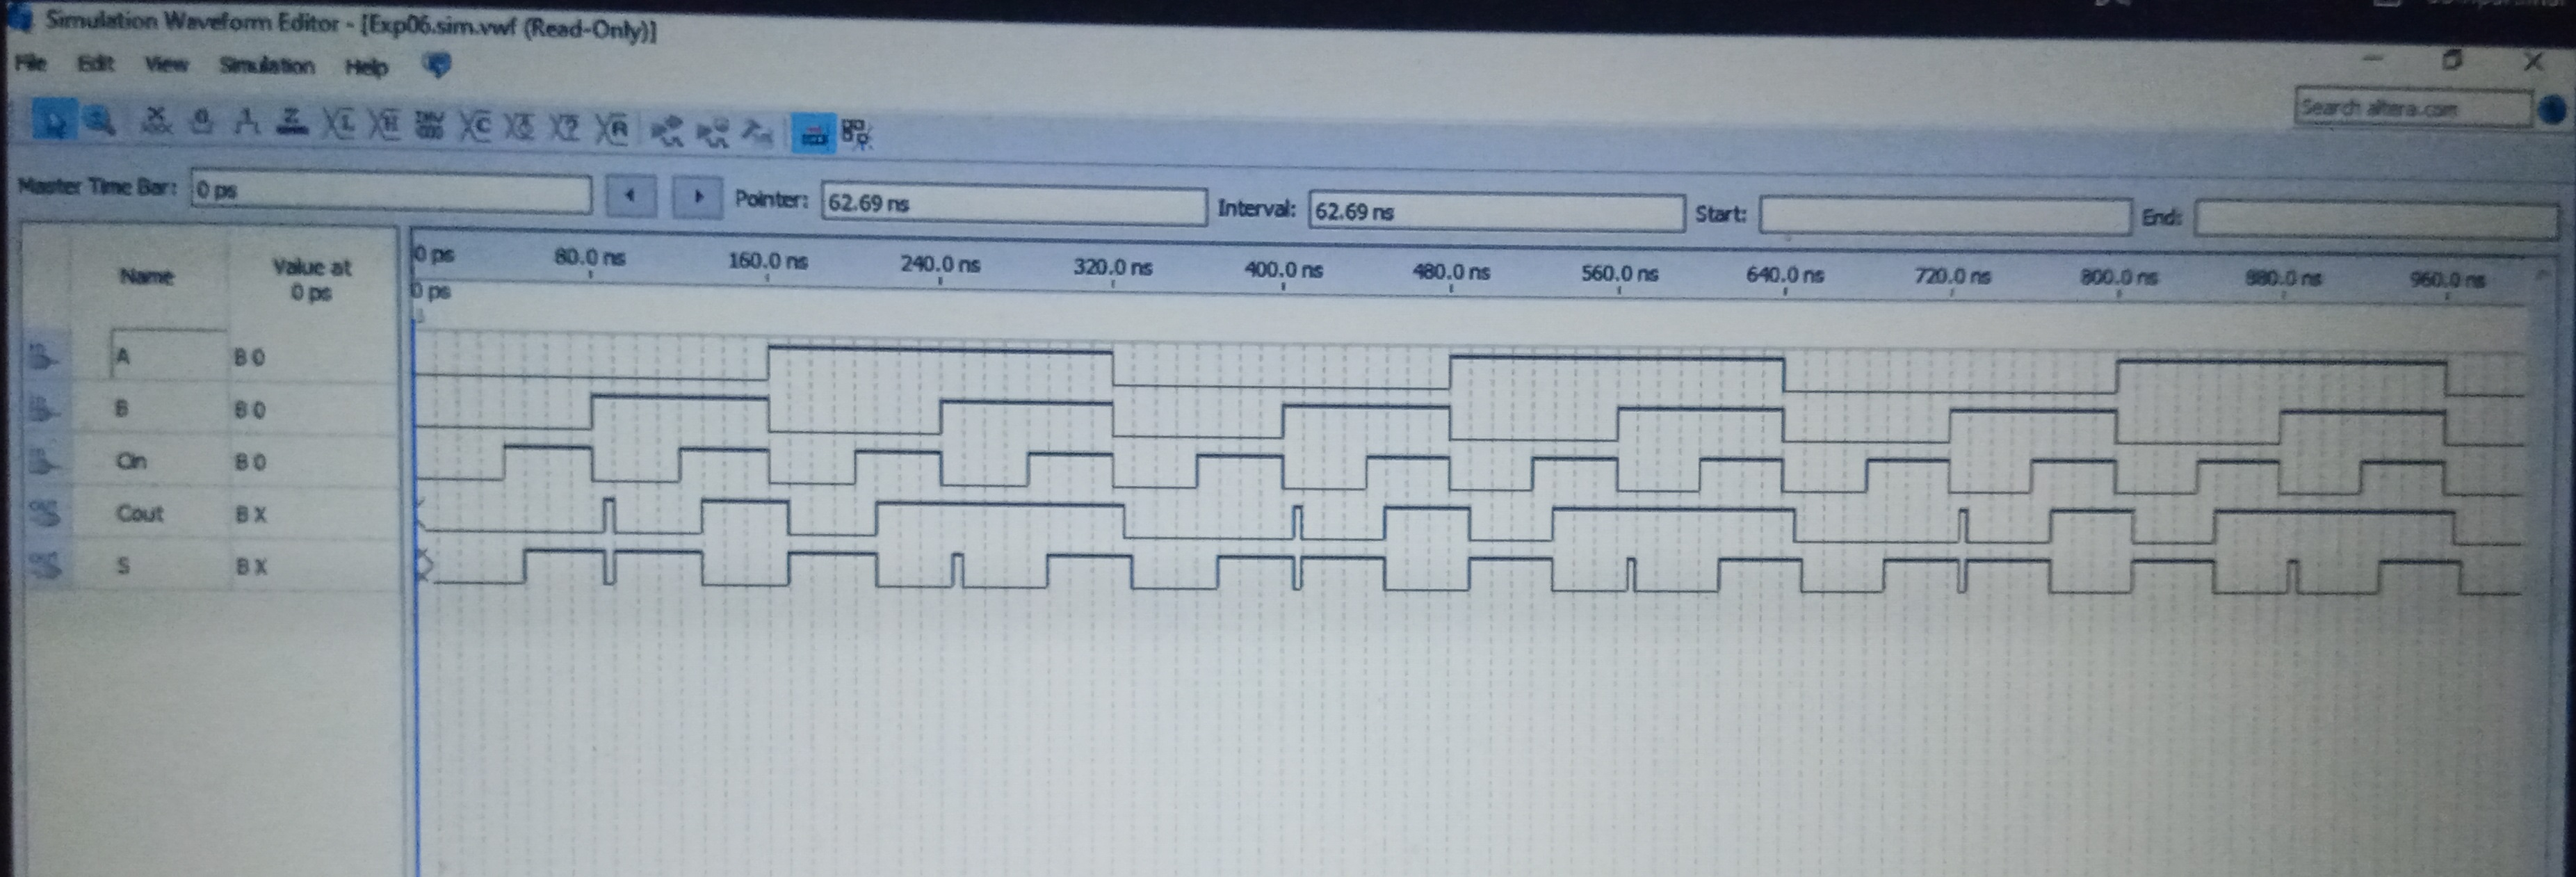
\includegraphics[width=0.9\textwidth]{Exp06/Images/2_2_Timing_Foto.jpg}
  \caption{Diagrama de Tempo do Somador implementado com \emph{SystemVerilog}}\label{fig:2_2_Timing_Foto.jpg}
\end{figure}


% 2.3
\subsection{Obtendo as funções booleanas para o decodificador com multiplexador}\label{sec:2.3}

Para o respectivo experimento utiliza-se uma implementação de decodificador com base no demultiplexador apresentado. Sendo em SystemVerilog expresso por:

\begin{center}
    \begin{lstlisting}[style={verilog-style}]
    module decod16(
        input [3:0] Escolha,
        output [15:0] Saida
        );

        assign Saida[0] = Escolha==4'd0? 1'b1 : 1'b0;
        assign Saida[1] = Escolha==4'd1? 1'b1 : 1'b0;
        assign Saida[2] = Escolha==4'd2? 1'b1 : 1'b0;
        ...
        assign Saida[14] = Escolha==4'd14? 1'b1 : 1'b0;
        assign Saida[15] = Escolha==4'd15? 1'b1 : 1'b0;
    endmodule
    \end{lstlisting}
    \label{code:full_adder}
\end{center}

Temos que a função analisada trata-se de:

$f(A,B,C,D,E,F,G)=FG+A.B.C.D.\overline{E}.\overline{F}.G+\overline{A}.\overline{B}.\overline{C}.\overline{D}.\overline{E}.\overline{F}.G+A.\overline{B}.\overline{C}.E.F.\overline{G}+\overline{A}.B.C.D.\overline{E}.F.\overline{G}+A.B.C.D.E.\overline{F}.\overline{G}+A.\overline{B}.\overline{C}.D.E.\overline{F}.\overline{G}$

A princípio define-se \textbf{A, B, C} e \textbf{D} como sendo os bits que irão compor o decodificador e \textbf{E, F, G} para o multiplexador. Também temos que \textbf{A} será o bit mais significativo e \textbf{G} o menos significativo.

Analisando somente os locais que possuem saída $1$, sua tabela verdade será descrita por:

\begin{table}[H]
    \centering
    \caption{Tabela Verdade para $f(A,B,C,D,E,F,G)$}
    \begin{tabular}{|c|c|c|c|c|c|c||c|}\hline
    \multicolumn{7}{|c||}{Entradas} & \multicolumn{1}{|c|}{Saídas} \\\hline
    \textbf{A} & \textbf{B} & \textbf{C} & \textbf{D} & \textbf{E} & \textbf{F} & \textbf{G} & \textbf{S} \\\hline
    0 & 0 & 0 & 0 & 0 & 0 & 1 & 1 \\\hline
    0 & 1 & 1 & 1 & 0 & 1 & 0 & 1 \\\hline
    1 & 0 & 0 & 1 & 1 & 0 & 0 & 1 \\\hline
    1 & 0 & 1 & * & 1 & 1 & 0 & 1 \\\hline
    1 & 1 & 1 & 1 & 0 & 0 & 1 & 1 \\\hline
    1 & 1 & 1 & 1 & 1 & 0 & 0 & 1 \\\hline
    * & * & * & * & * & 1 & 1 & 1 \\\hline
    \end{tabular}\label{tab:truth_table_full_adder}
\end{table}

Deve-se atentar ao fato de que pelo uso da expressão \textbf{FG} temos que para todas as combinações que possuem $F=1$ e $G=1$ o resultado será $1$, utilizando o processo de soma de produtos. Assim, temos que o circuito será descrito através da ferramenta Quartus II como:

\begin{figure}[H]
  \centering
  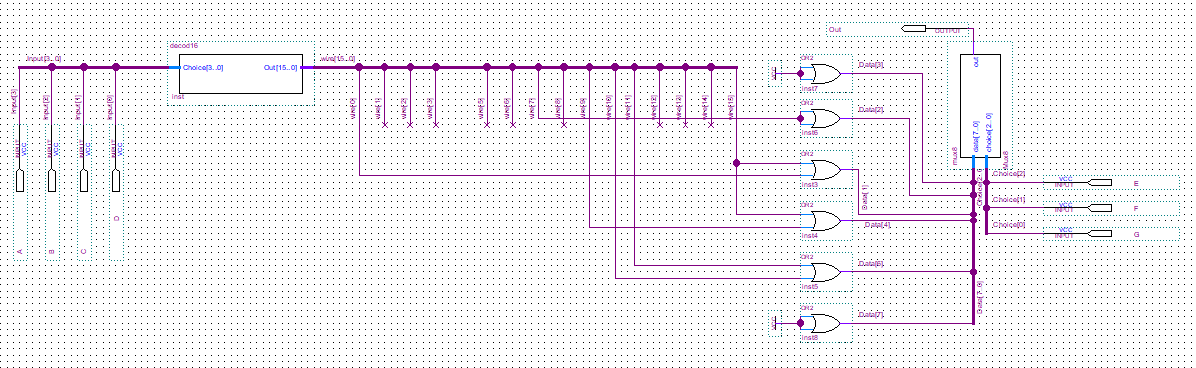
\includegraphics[width=0.9\textwidth]{Exp06/Images/2_3_Circuit.png}
  \caption{Decodificador e Multiplexador p/ Min Termos}\label{fig:2_3_Circuit.png}
\end{figure}

Simulando obtem-se em seu diagrama funcional:

\begin{figure}[H]
  \centering
  \includegraphics[width=0.9\textwidth]{Exp06/Images/2_3_Functional_Foto.jpg}
  \caption{Simulação Funcional 2.3}\label{fig:2_3_Functional_Foto.jpg}
\end{figure}

Observa-se que de fato para $F=1$ e $G=1$ temos que saída resulta em $1$, como previsto, além dos casos adicionais que compõe a função.

Simulando obtém-se para seu diagrama com análise de tempo:

\begin{figure}[H]
  \centering
  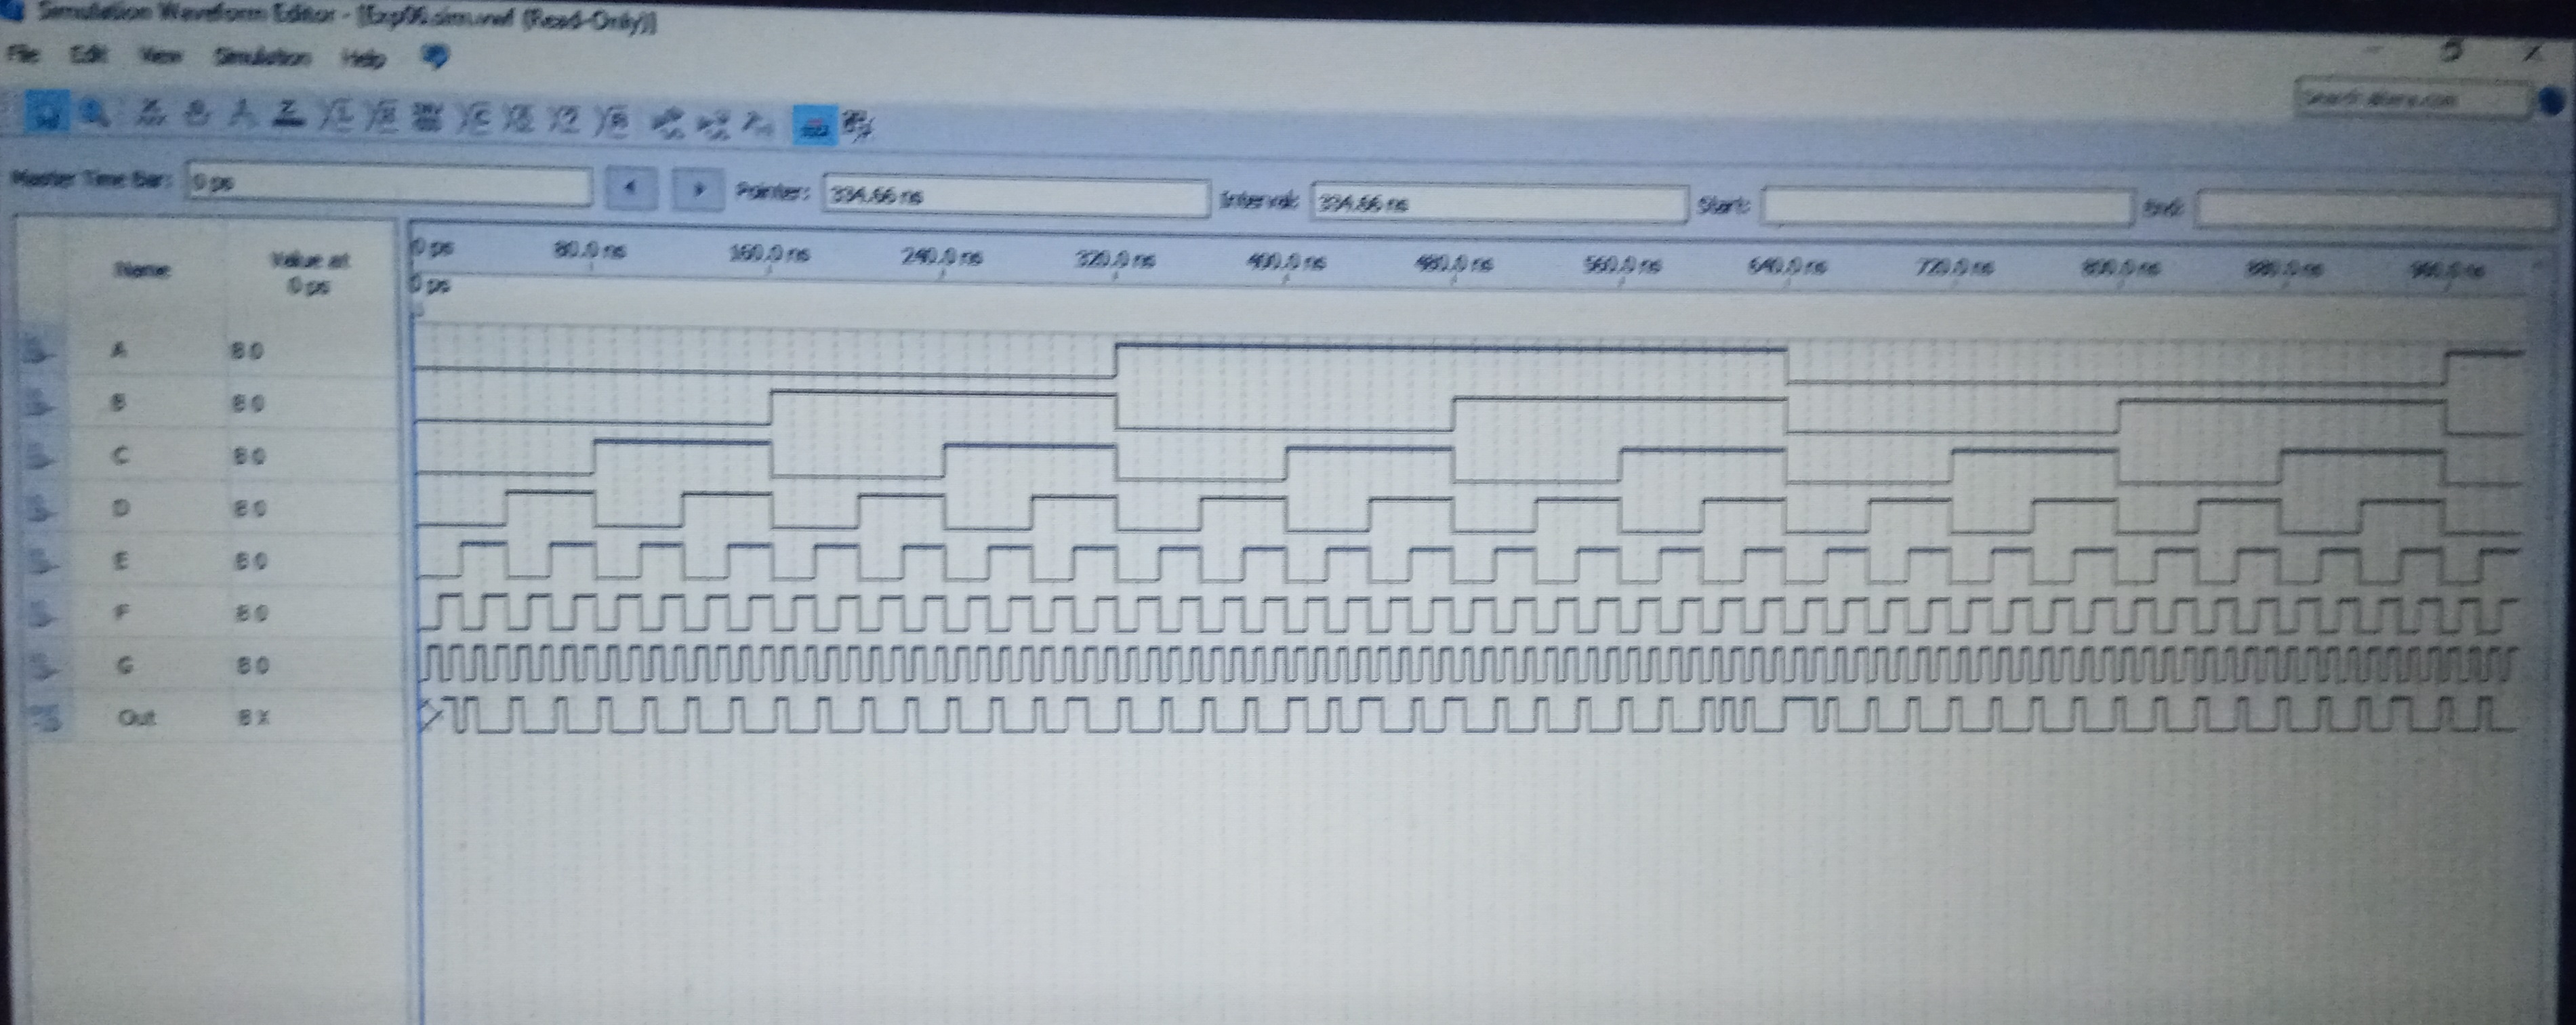
\includegraphics[width=0.9\textwidth]{Exp06/Images/2_3_Timing.jpg}
  \caption{Simulação Temporal 2.3}\label{fig:2_3_Timing_Foto.jpg}
\end{figure}

Observa-se que diferentemente dos experimentos prévios apesar de não haver Hazards de maneira tão evidente tem-se atrasos nos resultados a serem obtidos.

\section{Análise dos Resultados}\label{sec:resultados}

\subsection{Análise em~\ref{sec:2.1} e~\ref{sec:2.2}}\label{sec:analise2.1}

Dos experimentos \emph{2.1} e \emph{2.2} podemos fazer duas observações
interessantes e pertinentes.

A primeira observação é que o circuito criado em \emph{2.1} é praticamente o
mesmo que o feito em \emph{2.2}, hava vista que os diagramas
em~\ref{fig:2_1_Timing_Foto.jpg} e~\ref{fig:2_2_Timing_Foto.jpg} são iguais. E,
uma vez que \emph{2.1} e \emph{2.2} são iguais, vemos como uma linguagem de
descrição de hardware como o \emph{SystemVerilog} pode ser uma ferramenta útil,
pois o tempo de desenvolvimento dos dois circuitos é muito diferente. Enquanto
em um o programador precisa se preocupar em ligar corretamente todos os fios e
portas lógicas, no outro o programador só precisa especificar o comportamento
esperado do sistema, aumentando muito a produtividade no desenvolvimendo de
novos circuitos.

Outra observação pertinente de se fazer é que em ambos os circuitos há presença
de \emph{hazards}, que são ocasionados pelo fato de que os circuitos não serem
ideias (eles apresentam atrasos, fade-ins, fade-outs, etc.), e, dessa forma, é
importante notar que há momentos que os canais de saída do circuito final (os
pinos de \textbf{S} e \textbf{Cout}) apresentarão, nessa configuração, um
resultado errado durante um curto período de tempo.


\subsection{Análise em~\ref{sec:2.3}}\label{sec:analise2.4}

Apesar do experimento \ref{sec:2.3} não possuir Hazards evidentes como os outros observados, deve-se atentar ao tempo de propagação. Para visualização do experimento utilizou-se um período de $5ns$, para uma análise funcional não temos muitos problemas na adoção deste período, contudo, é errôneo a adoção de um período tão pequeno em projetos práticos, este problema é extremamente evidente na simulação temporal onde temos que a cada novo estado a saída capta o resultado anterior, tal fato é o que justifica uma longa indefinição inicial.

Para este relatório apesar de errônea esta adoção, escolheu-se para a visualiazação de todos os resultados possíveis e também sermos capazes de analisar o respectivo erro e abordá-lo.

\section{Conclusão}\label{sec:Conclusao}

O presente relatório foi capaz de além da utilização de multiplexadores, demultiplexadores e decodificadores para a geração de variados tipos de circuitos, como também pudemos ser capazes de analisar os erros associados a suas composições e a importância de ser definido um tempo de mudança ideal para circuitos, caso contrário poderá ser grande o erro obtido nos resultados.

Importante mencionar que circuitos como ``\emph{half-adder}'' e `` \emph{full-adder}'' são de extrema importância para a computação, por serem estes elementos que compõe componentes eletrônicos como processadores, pois, com eles somos capazes de contar tempo passado, ciclos realizados, deslocamento entre instruções, assim como também operações de soma no geral, porém, não limita-se a somente as possibilidades mencionadas.


\nocite{*}
\bibliographystyle{sbc}
\bibliography{relatorio}  %Aqui é a definição do arquivo .bib a ser usado pelas referências


\newpage
% Colocar aqui apenas as respostas dos itens da Auto-Avaliação
\section*{Auto-Avaliação}

Respostas:

\begin{table}[H]
      \begin{tabular}{|c|c|} \hline
      \textbf{Questão} & \textbf{Resposta}\\
      \hline
      1  & V \\ \hline
      2  & V \\ \hline
      3  & F \\ \hline
      4  & V \\ \hline
      5  & F \\ \hline
      6  & V \\ \hline
      7  & V \\ \hline
      8  & F \\ \hline
      9  & V \\ \hline
      10 & F \\ \hline
      11 & V \\ \hline
      \end{tabular}
\end{table}


\end{document}
